\documentclass[tikz,border=20pt]{standalone}
\usepackage{mathptmx}
\usepackage{tikz}
\usetikzlibrary{arrows.meta, calc}

\tikzset{
  extentity/.style={rectangle, draw=black, line width=1.5pt,
    minimum width=2.8cm, minimum height=0.9cm,
    font=\bfseries\small, align=center},
  process/.style={circle, draw=black, line width=1.5pt,
    minimum size=3.2cm, font=\bfseries\small, align=center},
  flow/.style={->, >=Stealth, line width=1pt},
  flabel/.style={font=\footnotesize, align=center, inner sep=2pt,
    fill=white, text width=2.4cm}
}

\begin{document}
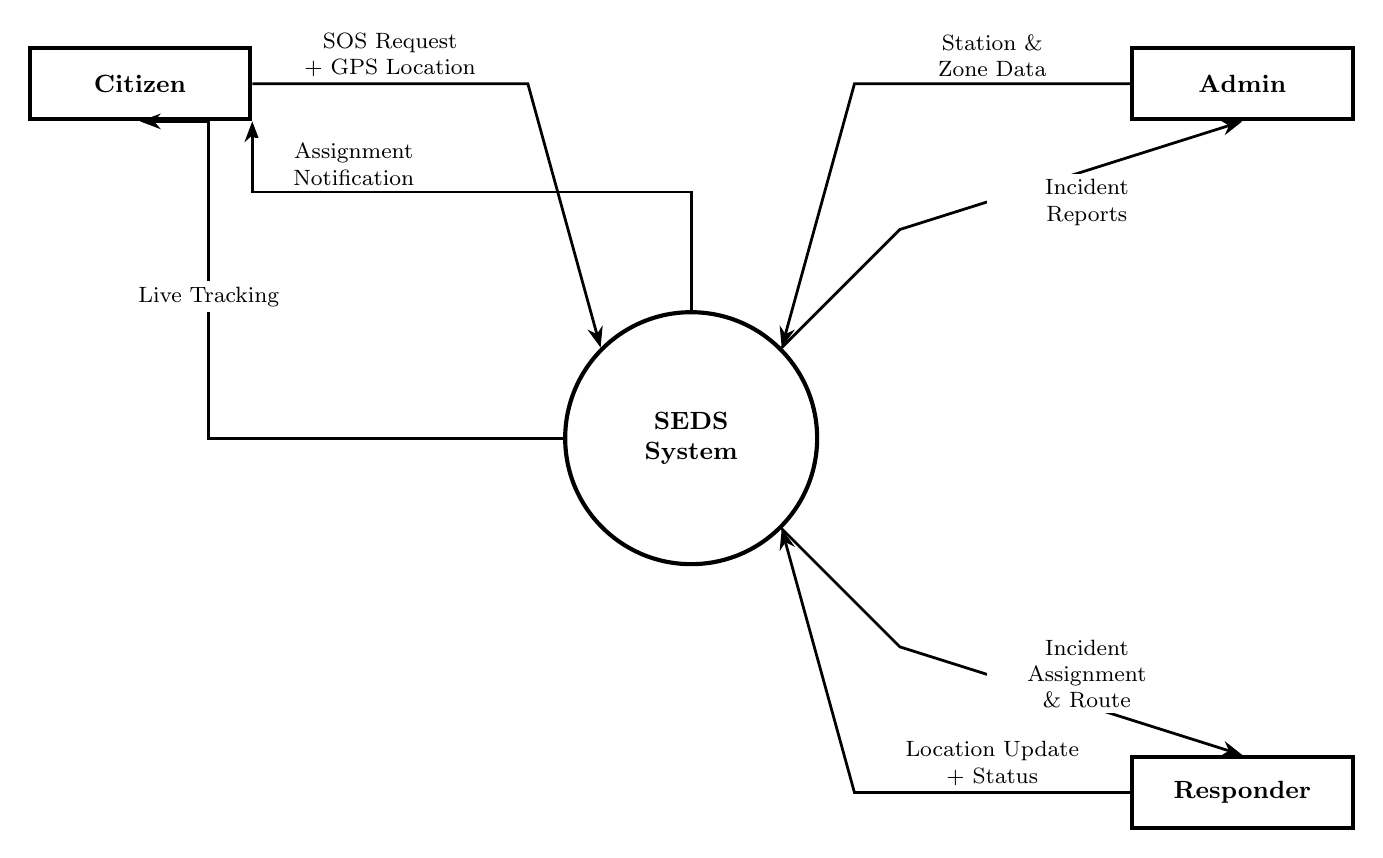
\begin{tikzpicture}

% Central process
\node[process] (seds) at (0,0) {SEDS\\System};

% External entities at four corners
\node[extentity] (citizen)   at (-7,  4.5) {Citizen};
\node[extentity] (admin)     at ( 7,  4.5) {Admin};
\node[extentity] (responder) at ( 7, -4.5) {Responder};

% ── Citizen ──────────────────────────────────────────────
\draw[flow] (citizen.east)  -- node[flabel, above, sloped] {SOS Request\\+ GPS Location} ++(3.5,0) -- (seds.north west);
\draw[flow] (seds.north)    -- ++(0,1.5) -| (citizen.south east)
  node[flabel, midway, above right] {Assignment\\Notification};
\draw[flow] (seds.west)     -- ++(-2.5,0) -- ++(-2,-0) |- (citizen.south)
  node[flabel, near start, below] {Live Tracking};

% ── Admin ──────────────────────────────────────────────
\draw[flow] (admin.west)    -- node[flabel, above, sloped] {Station \&\\Zone Data} ++(-3.5,0) -- (seds.north east);
\draw[flow] (seds.north east) -- ++(1.5,1.5) -- (admin.south)
  node[flabel, near start, right] {Incident\\Reports};

% ── Responder ──────────────────────────────────────────────
\draw[flow] (responder.west) -- node[flabel, above, sloped] {Location Update\\+ Status} ++(-3.5,0) -- (seds.south east);
\draw[flow] (seds.south east) -- ++(1.5,-1.5) -- (responder.north)
  node[flabel, near start, right] {Incident\\Assignment\\\& Route};

\end{tikzpicture}
\end{document}
